Matematický model, ktorý opisuje bioreaktor je nelineárny model. To znamená, že odozva systému je rôzna pre rovnakú veľkosť skokovej zmeny.
% RP: Trocha neuplna veta. ``odozva systému je rôzna pre rovnakú veľkosť skokovej zmeny'' toto je pravda pre rozne pociatocne podmienky a treba to jasne napisat
Túto nelinearitu si možno všimnúť na Obr. \ref{fig:1}.
% RP: Jedna veta nemoze povedat ``pozrite sa na obrazok'' a druha uz predpokladat, ze z obrazka citatel ``najedol''. Obrazok treba popisat. Napr. ``na obrazku je ukazany priebeh vystupu...'' Aka simulacia bola vlastne urobena? Aky model? Ake pociatocne podmienky? Ake vstupy?
Ďalej si môžme všimnúť prudký narást koncentrácie produktu na počiatku, ktorý bol spôsobený nadbytkom biomasy a malým množstvom substrátu v systéme.
% RP: Myslim, ze na ``male mnozstvo substratu'' nema vplyv na produkt. Nakoniec ``s'' sa v rovnici (7) nenachadza.
Po ustálení dynamika produtku pripomímna systém 1. rádu. Na druhej strane v dynamike tvorby biomasy sa prejavuje nestabilná nula (menšie podkmity), ktoré sú spôsobené veľkou časovou konštantou tvorby biomasy a malou časovou konštantou odtoku suspenzie.
% RP; Odtok suspenzie nie je stav, takze nema casovu konstantu. Tento efekt by sa dal vysvetlit krajsie...napisem to len narychlo: v dosledku zvysenie prietoku latky cez reaktor, pritecie viac substratu, cim sa zvysi jeho koncentracia; koncentracia mikroorganizmov sa ale znizi; nasledne zvysena koncentracia substratu podpori rast biomasy a tym sa aj koncetracia biomasy zacne zvysovat.
V dynamike substrátu sa zasa prejavuje stabilná nula, ktorá opäť súvisí s rýchlym prítokom česrstvého média a pomalšou spotrebou na tvorbu biomasy a produktu.
% RP: spell check ``česrstvého''

\begin{figure}
	\centering
	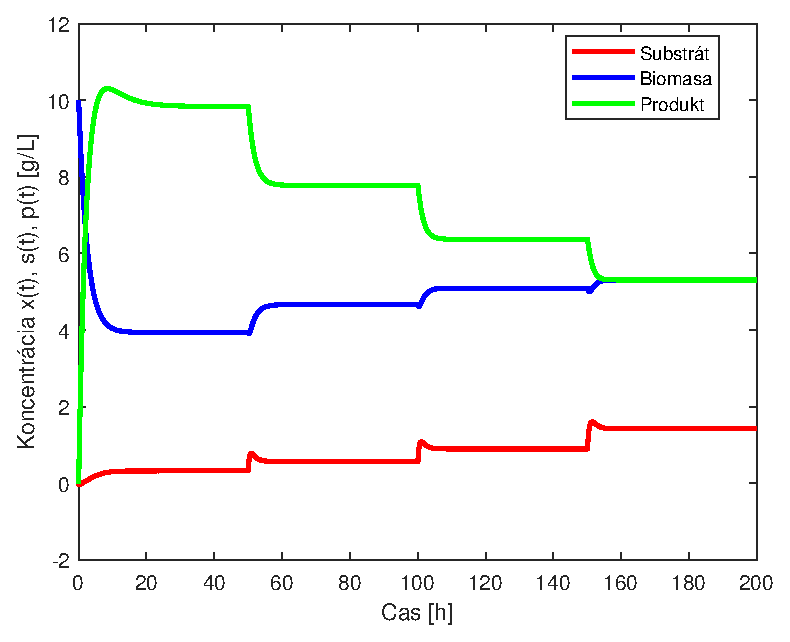
\includegraphics[width=.7\linewidth]{images/step_change}
	\caption[]{Viacnásobná skoková zmena rýchlosti riedenia $D$ pri začiatočných podmienkach $p_0 = s_0 = 0, x_0 = 10 gL^{-1}$.}
	% RP: Popis obrazku musi popisat, co je na obrazku ukazane. Ja tam ``viacnásobnú skokovú zmenu rýchlosti riedenia'' nevidim.
	% RP: Opat su tu ``kurzivove'' jednotky.
	\label{fig:1}
\end{figure}

Režim fungovania bioreaktora má významný vplyv na dynamiku celého systému a pri určitých podmienkach Monod model a model s inhibíciou môžu vykazovať rovnaké správanie, presne ako je tomu na Obr. \ref{fig:1}. Avšak, tieto modely sa odlišujú vo formulácii špecifickej rýchlosti rastu, ktorý má zásadný vplyv na dynamiku systému. Ako vidno na Obr. \ref{fig:2} pri Monod modely
% RP: spell check ``modely''
sa špecifická rýchlosť rastu limitne blíži ku maximálnej špecficikej rýchlosti rastu, zatiaľ čo model s inhibícou dosahuje svoje maximum v bode $S^{*} = \sqrt{K_M K_i}$.
% RP: Nie je jasne co je vlastne ukazane na obrazku. Nikto si len tak ``z prsta nevycuca'' ze ukazujete ustalene stavy. Tie musite predstavit na zaklade modelu.
Pri nesprávne zvolených pracovných podmienkach, či už počiatočných podmienkach systému, koncentrácie čerstvého substrátu alebo rýchlosti riedenia, model s inhibíciou bude vykazovať diametrálne odlišné správanie od Monod modelu, ako to je zobrazené na Obr. \ref{fig:3}.
% RP: Opat treba obrazok popisat. Najlepsia zasada je aby plocha obrazku zodpovedala ploche textu, ktory obrazok opisuje.
% RP: Hodilo by sa tu opisat, co sa deje v tychto dvoch reaktoroch a takisto by sa citatel mal po prvykrat dozvediet, ze existuje nieco ako washout (stav vymytia?) kedy je prevadzka reaktora nenavratne narusena.

\begin{figure}
	\centering
	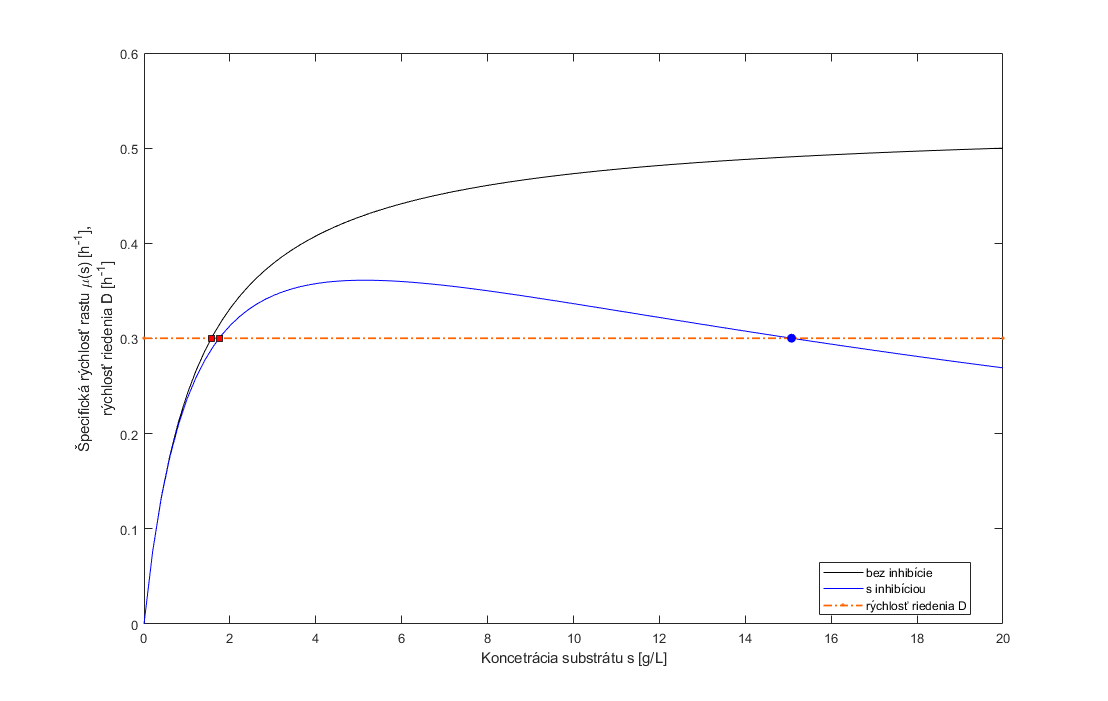
\includegraphics[width=.7\linewidth]{images/spec_grow_rate_comparison}
	\caption[]{Porovnanie priebehu špecifickej rýchlosti rastu Monod modelu (červená) a modelu s inhibíciou (modrá). Červeným štvorčekom sú označené nenulové stabilné ustálené stavy, modrou guličkou je označený nestabilný stav.}
	% RP: Legenda mi pride nekonzistentna. Dal by som odtial prec ``rychlost riedenia D'' a skor uviedol v popise obrazku, ze bodkociarkovanou ciarou je znazornena zvolena rychlost riedenia D = 0.3h^-1
	\label{fig:2}
\end{figure}

\begin{figure}
	\begin{subfigure}{.5\textwidth}
		\centering
		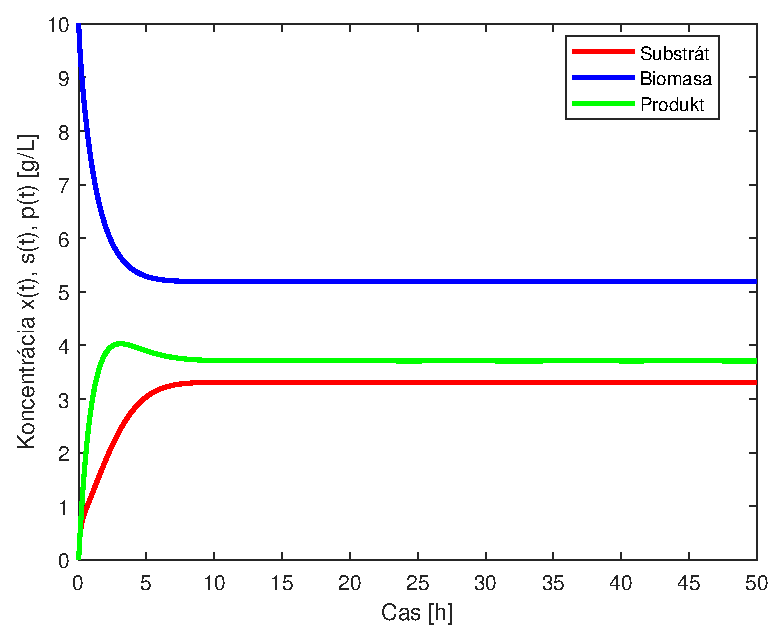
\includegraphics[width=1\linewidth]{images/dyn_Monod}
		\caption[]{Monod model}
	\end{subfigure}
	\begin{subfigure}{.5\textwidth}
		\centering
		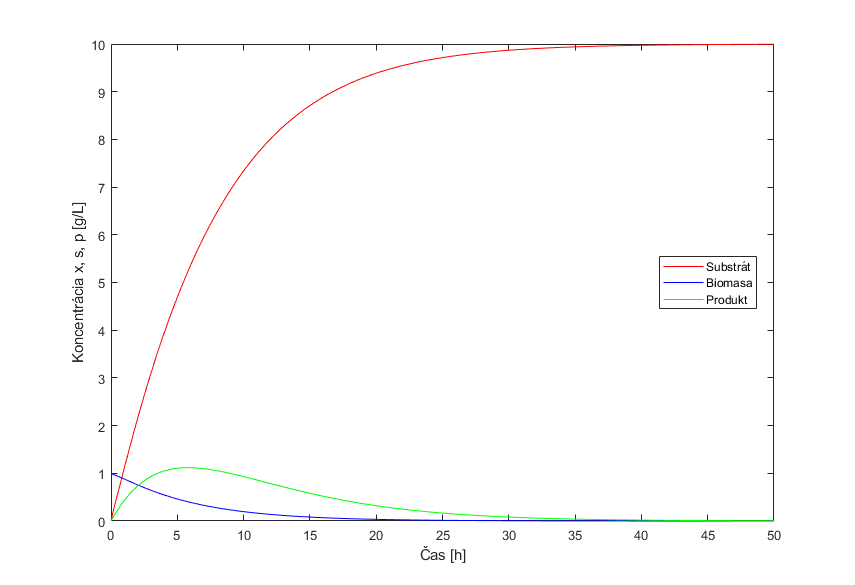
\includegraphics[width=1\linewidth]{images/dyn_inhb}
		\caption[]{Model s inhibíciou}
	\end{subfigure}
	\caption{Porovnanie dynamiky modelov pri rovnakých pracovných podmienkach.}
	\label{fig:3}
\end{figure}
